%% This is the Project Description FOr IHCI group Project
%%
%% Group Members:
%%% Shivoy Arora
%%% Tushar Kumar
%%% Gaurav Gupta
%%% Ayush
%%% Manish
%%% Ankit Kumar Pal

\documentclass[acmtog]{acmart}
% \documentclass[manuscript,screen,review]{acmart}

\AtBeginDocument{%
  \providecommand\BibTeX{{%
    \normalfont B\kern-0.5em{\scshape i\kern-0.25em b}\kern-0.8em\TeX}}}


\usepackage[utf8]{inputenc}

\title{HCI Project}

%%% Authors
\author{Shivoy Arora}
\email{shivoy21420@iiitd.ac.in}

\author{Tushar Kumar}
\email{tushar21212@iiitd.ac.in}

\author{Gaurav Gupta}
\email{gaurav21148@iiitd.ac.in}

\author{Ayush}
\email{ayush20501@iiitd.ac.in}

\author{Manish}
\email{manish21164@iiitd.ac.in}

\author{Ankit Kumar Pal}
\email{ankit21132@iiitd.ac.in}

\date{March 2022}

\begin{document}

\maketitle

% Problem Definition
\section{PROBLEM DEFINITION AND IDENTIFYING STAKEHOLDERS}

\subsection{Define the problem}
We face a lot of issues in our daily life. Some of them are personal while some are social. Social issues need some kind of political involvement and administrative assistance from the government side. But in our daily life, there is no such place or way by which we can directly approach our political representatives. Maybe some sort of solution is available but it is not within the reach of the common man. There is no transparency between people and political leaders. Most of the people don’t know about their political representative and their approach to solving an issue. We find it a very important issue we are dealing with today.

\subsection{Background of the Problem and Motivation}
One of our project group members, who live in a semi-remote area told us about the problem of bad road conditions in his area. Due to this, there were no means of transport and accidents had turned very common for them. One day some people of the society gathered to complain against it as it was making their normal life difficult. So they decided to meet their MLA to report about the bad road conditions. The MLA listened to them and asked to go to the Municipality Office, as they are responsible for this. Then they visited the Municipality Office where they didn’t get proper assistance. It took more than three months and a lot of effort to get the work done. After listening to him we thought to design something that will “Repair the road between the people and the government”.

\subsection{Stakeholders and their role}
\subsubsection{Common People}
As in politics, common people play a significant role. Various issues are faced by people which need political support get resolve
\subsubsection{Political representatives}
Political leaders (, i.e. MPs, MLAs, and counsellors) are at the center of this issue as they are the only ones who can resolve the issue raised
\subsubsection{Government officials}
Any order or solution of an issue given by a political representative is implemented by government officials
\subsubsection{Media}
The role of media is to check the accountability and issue-resolving strategy of the government.

\subsection{What other products exist which are trying to solve similar problems?}
\begin{enumerate}
    \item Complain register/box available at the residence of political leaders and government offices.
    \item Government websites of different departments.
    \item Government dictionary for all govt. websites: - \url{https://igod.gov.in/}
    \item Publishing an issue in media that makes it more famous. 
\end{enumerate}

\subsection{Limitation of current products}
Complain registers are sometimes missing or hard to get from the corresponding official. It is time-consuming. In some places, such complaint systems don’t have any value.
Government websites need some previous knowledge to deal with them. These are very slow due to low maintenance.
Government dictionaries are too much hard to be handle as they have thousands of websites. It causes a cognitive load on the user while using them.
Publishing any issue in media is a long process and it takes more than the desired time to get resolved.

\subsection{How could/would your solution be novel?}
In our design we will provide the following facilities which make the process easier:
\begin{enumerate}
    \item User will enter their issue and their location. Our program will find the authorized political leader or govt. official available at that time to solve that issue.
    \item Our program also provides the link to a suitable website if they want the solution to be online.
    \item A notification has been sent to the concerned political leader or govt. official about the issue which has been raised in their area.
    \item There is a profile system for every political representative (describing the no. of issues solved by them) so that users can find the accountability and efficiency of a representative.
    \item  User will get notified about the latest policies made by the government.
    \item Program will provide assistance to users while applying for some important documents (such as VOTER ID CARD, AADHAAR CARD, DRIVING LICENSE, etc.) 
    \item Our program have some stuff available that help user to understand the political structure and function of the country.
    \item Our program will make the user aware of their rights as stated by the government.
\end{enumerate}

\subsection{Challenges we will face}
\begin{itemize}
    \item There is no correct contact information available about all the political leaders.
    \item Leaders and government officials keep changing and there is no place where all these updates are available
    \item Many of government websites don’t give us access.
\end{itemize}

\section{REQUIREMENT GATHERING}
We have tried to reach the audience by the means of a google from which contained some questions related to the issue we are solving. We have got the following analysis

\begin{figure}[H]
    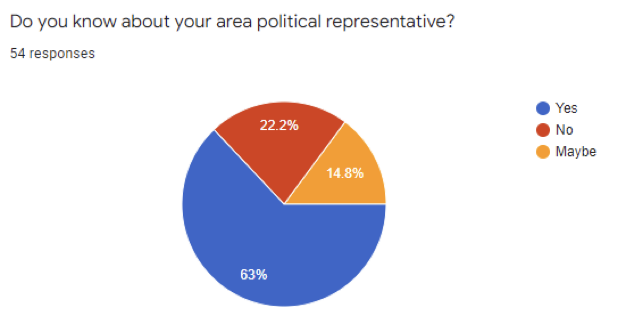
\includegraphics[width=8cm]{Resources/q1}
    \caption{Question 1}
    \label{fig:q1}
    \Description{Do you know about your area's political representative}
\end{figure}

In this question, we ask people whether they are familiar with (or know) their regional politics. According to the responses we come to know that majority of people are known to their political representative. But there is a group of people (approx. 37\%) who don’t know about their political leader. Our task is to make all people aware of their political representative.

\begin{figure}[H]
    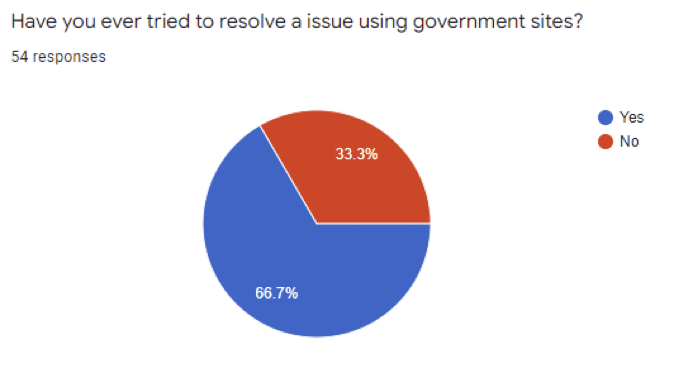
\includegraphics[width=8cm]{Resources/q2}
    \caption{Question 2}
    \label{fig:q2}
    \Description{Have you ever tries to resolve a issue using government sites}
\end{figure}

From the above data we analyse that majority of people are engaged somehow in solving any issue either social or personal which need the interference of political leaders.

\begin{figure}[H]
    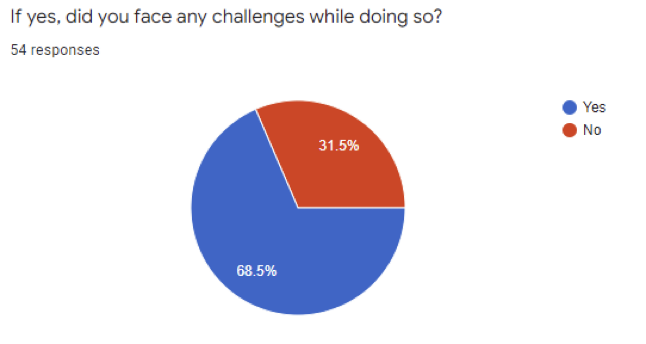
\includegraphics[width=8cm]{Resources/q3}
    \caption{Question 3}
    \label{fig:q3}
    \Description{If yes, did you face any challenges while doing it}
\end{figure}

The above data clearly states that the peoples who are engaged in solving any issue, a huge majority of people face challenges while resolving it. This is our main aim to make this process of solving issues simpler so people don’t face too many challenges.


\begin{figure}[H]
    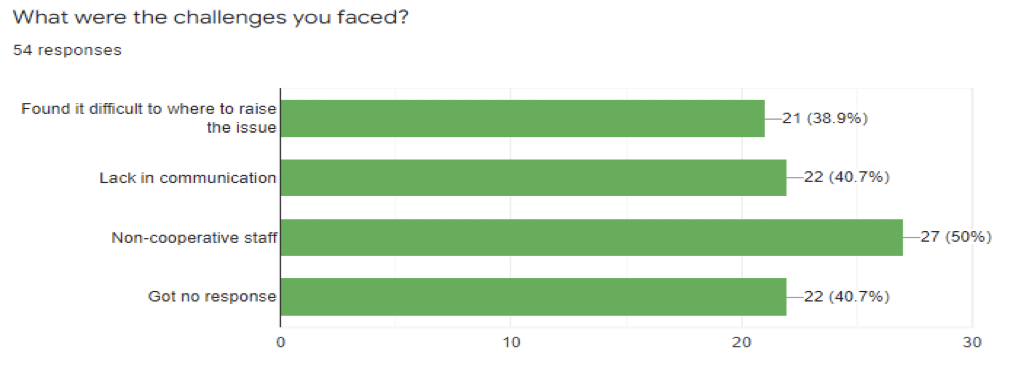
\includegraphics[width=8cm]{Resources/q4}
    \caption{Question 4}
    \label{fig:q4}
    \Description{What were the challenges you faced}
\end{figure}

In continuation of the above ques, we give some general challenges which were faced. Most people face all of the provided issues. But the issue of non-cooperative staff is faced by most of them. This challenge arises because of corruption in our system and there is no cross-checking and transparency. People not getting any response regarding their issue is also because of the same reason.

\begin{figure}[H]
    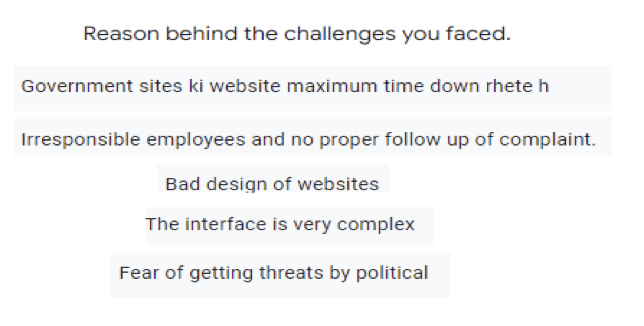
\includegraphics[width=8cm]{Resources/q5}
    \caption{Question 5}
    \label{fig:q5}
    \Description{Reasons behind the challenges faced}
\end{figure}

Here are some other reasons for the challenges faced by the people while solving an issue. We analyse that most people face problems while using a government website. This is because of the bad design and complex interface of websites. 

\begin{figure}[H]
    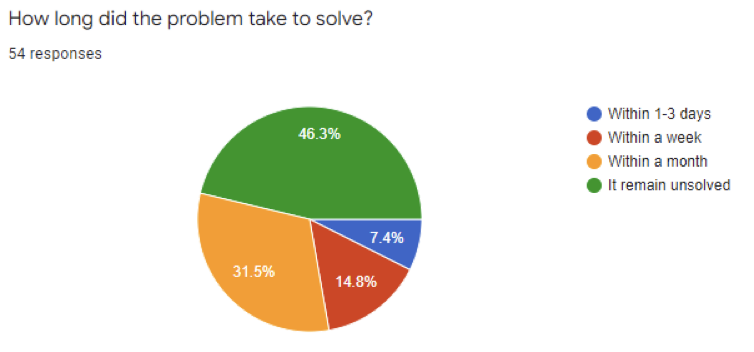
\includegraphics[width=8cm]{Resources/q6}
    \caption{Question 6}
    \label{fig:q6}
    \Description{How long did the problem take to solve}
\end{figure}

We ask the audience to respond to the ques about the time which it takes to resolve an issue. Approx. half of them responded that their issue remains unsolved or it may take up to a month to solve the issue.

\begin{figure}[H]
    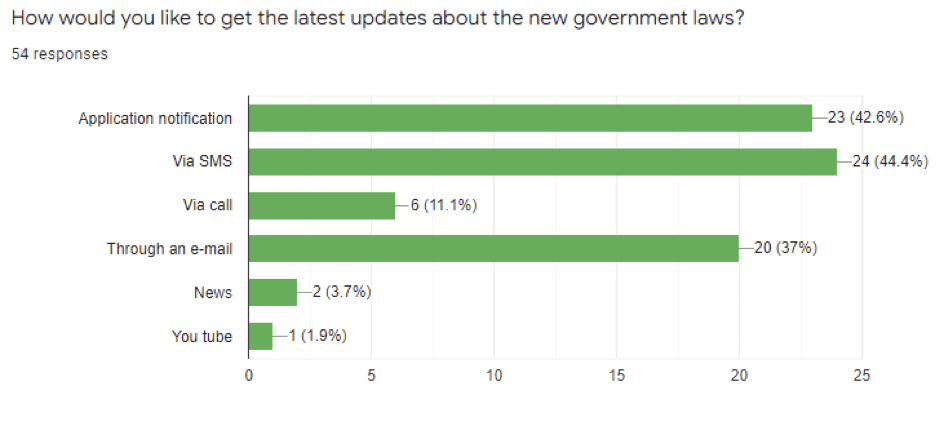
\includegraphics[width=8cm]{Resources/q7}
    \caption{Question 7}
    \label{fig:q7}
    \Description{How would you like to get the latest updates about the new government laws}
\end{figure}

The above poll shows that most people are interested to get an update on all the policies and decisions made by the government. Most of them wanted to get notified through SMS on their phone or by the application notification of our program. Those who spend their time on PCs and laptops want to get notified through E-mail.

\begin{figure}[H]
    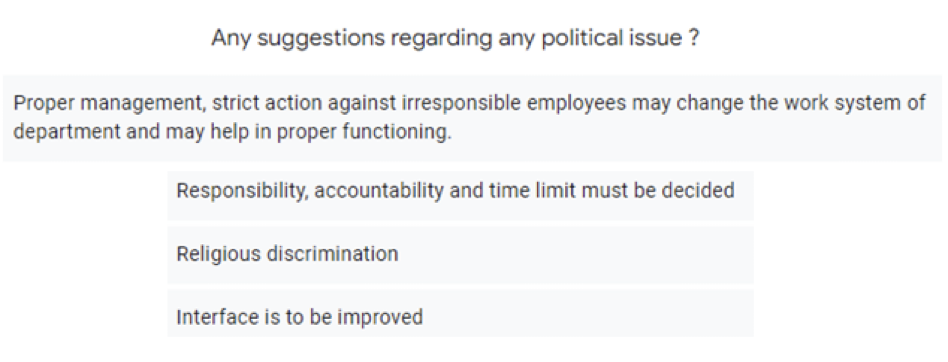
\includegraphics[width=8cm]{Resources/q8}
    \caption{Question 8}
    \label{fig:q8}
    \Description{Suggestions}
\end{figure}

Here are some other suggestions related to our program. We will take up these suggestions very strongly while designing our program
\end{document}
